\documentclass[tikz,border=8pt]{standalone}
% Shared look for every TikZ diagram. Load with \input{../../tools/tikz-style.tex}
\usepackage[sfdefault]{roboto}
\usetikzlibrary{arrows.meta, positioning, shapes.geometric, calc, fit, backgrounds}
\definecolor{cblue}{HTML}{4C78A8}
\definecolor{corange}{HTML}{F58518}
\definecolor{cgreen}{HTML}{54A24B}
\definecolor{cred}{HTML}{E45756}
\definecolor{cpurple}{HTML}{B279A2}
\definecolor{cgrey}{HTML}{6B6B6B}
\tikzset{
  every picture/.style={font=\sffamily, line width=1.2pt},
  box/.style={draw=#1, fill=#1!12, rounded corners=4pt, align=center, inner sep=7pt, minimum height=1.1cm},
  box/.default=cgrey,
  arrow/.style={-{Stealth[length=3mm]}, draw=cgrey, line width=1.4pt},
  title/.style={font=\sffamily\bfseries\Large},
  note/.style={font=\sffamily\small, text=cgrey, align=center},
}
\AtBeginDocument{\hyphenpenalty=10000 \exhyphenpenalty=10000}

% The offset point (MR eq. 13.19-13.21; Paden V.B.2), drawn 8 cm per metre for the robot and 10 cm per m/s for speeds.
% A point a distance d ahead of the axle midpoint moves at v ahead plus d*w to the left; at d = 0 the left part is 0.
% Start of the run: wanted velocity of P = (0.5, -0.1) m/s, so v = 0.5 m/s and w = -0.1 / 0.2 = -0.5 rad/s.
\begin{document}
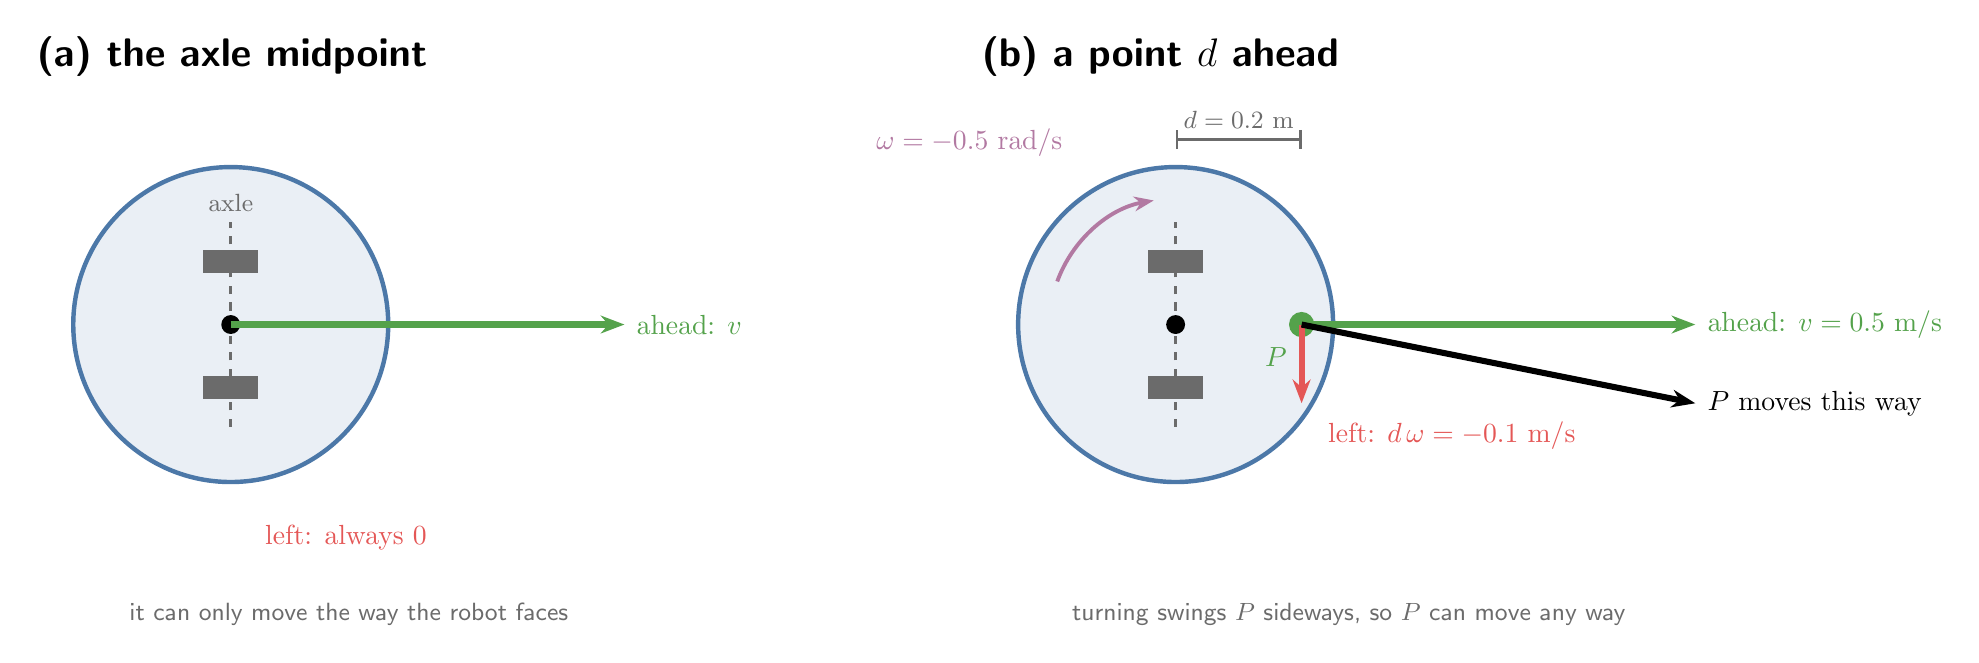
\begin{tikzpicture}[every node/.append style={font=\normalsize},
  vel/.style={-{Stealth[length=3mm]}, line width=2.2pt}]
  % ---------- (a) midpoint ----------
  \begin{scope}
    \node[title, anchor=west] at (-2.6,3.4) {(a) the axle midpoint};
    \draw[draw=cblue, fill=cblue!12, line width=1.6pt] (0,0) circle (2);
    \fill[cgrey] (-0.35,0.65) rectangle (0.35,0.95); \fill[cgrey] (-0.35,-0.95) rectangle (0.35,-0.65);
    \draw[cgrey, line width=1pt, dashed] (0,-1.3) -- (0,1.3) node[above, font=\small] {axle};
    \fill[black] (0,0) circle (0.12);
    \draw[vel, cgreen] (0,0) -- (5,0) node[right, align=left] {ahead: $v$};
    \node[cred, align=left, anchor=west] at (0.3,-2.7) {left: always 0};
    \node[note, anchor=north] at (1.5,-3.4) {it can only move the way the robot faces};
  \end{scope}
  % ---------- (b) offset point ----------
  \begin{scope}[xshift=12cm]
    \node[title, anchor=west] at (-2.6,3.4) {(b) a point $d$ ahead};
    \draw[draw=cblue, fill=cblue!12, line width=1.6pt] (0,0) circle (2);
    \fill[cgrey] (-0.35,0.65) rectangle (0.35,0.95); \fill[cgrey] (-0.35,-0.95) rectangle (0.35,-0.65);
    \draw[cgrey, line width=1pt, dashed] (0,-1.3) -- (0,1.3);
    \fill[black] (0,0) circle (0.12);
    \draw[cgrey, line width=1pt, |-|] (0,2.35) -- node[above, font=\small] {$d = 0.2$ m} (1.6,2.35);
    \fill[cgreen] (1.6,0) circle (0.16); \node[cgreen, anchor=north east] at (1.55,-0.15) {$P$};
    \draw[vel, cgreen] (1.6,0) -- (6.6,0) node[right, align=left] {ahead: $v = 0.5$ m/s};
    \draw[vel, cred] (1.6,0) -- (1.6,-1.0); \node[cred, anchor=north west] at (1.8,-1.1) {left: $d\,\omega = -0.1$ m/s};
    \draw[vel, black] (1.6,0) -- (6.6,-1.0) node[right] {$P$ moves this way};
    \draw[cpurple, line width=1.4pt, -{Stealth[length=2.5mm]}] (160:1.6) arc (160:100:1.6);
    \node[cpurple, anchor=south east] at (-1.3,2.0) {$\omega = -0.5$ rad/s};
    \node[note, anchor=north] at (2.2,-3.4) {turning swings $P$ sideways, so $P$ can move any way};
  \end{scope}
\end{tikzpicture}
\end{document}
